%% ----------------------------------------------------------------
%% Results.tex
%% ---------------------------------------------------------------- 
\chapter{Results And Discussion} \label{Chapter:Results}

\section{VGG Architecture Comparisons}
To estimate the impact of the backbone network and the side-network, each RetinaNet proposed architecture gets deployed on each VGG network separately. \fref{fig7} and \ref{fig8} show how AP and the F1-score scales with the depth of the backbone network.   

\begin{figure}[!htb]
  \centering
  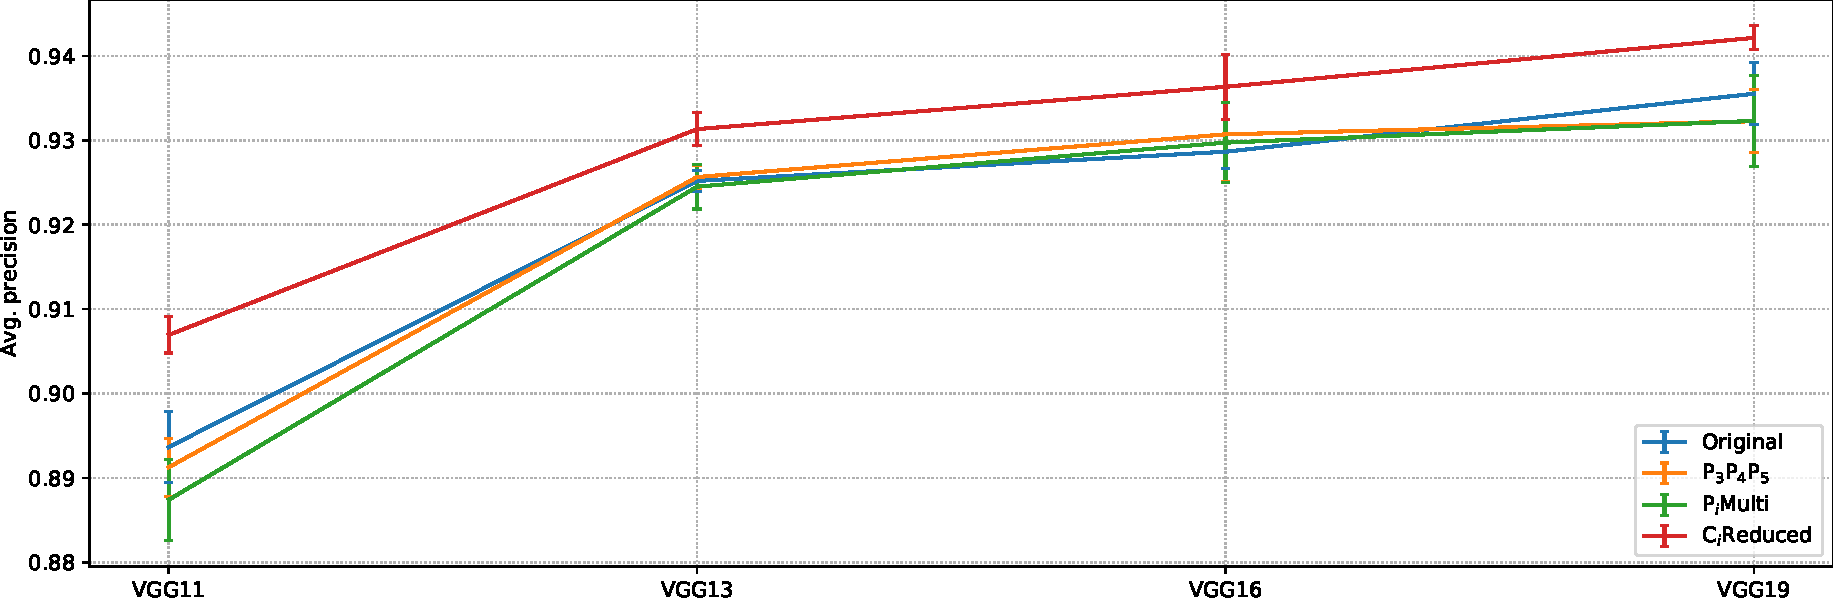
\includegraphics[width=\textwidth]{figures/ch3/fig7.pdf}
  \caption{Comparative results of Avg. Precision versus the four VGG models, for each proposed RetinaNet model. Results were averaged over 10 times.}
  \label{fig7}
\end{figure}

\begin{table}[!htb]
  \centering
  \resizebox{0.75\textwidth}{!}{
  \begin{tabular}{ccccc}
  \toprule
  \textbf{Avg. Precision} & \textbf{VGG11} & \textbf{VGG13} & \textbf{VGG16} & \textbf{VGG19} \\
  \midrule
  Original (202)								&	0.894$\pm$0.004		&	0.925$\pm$0.001		& 	0.929$\pm$0.002		&	0.936$\pm$0.004\\
  $\text{P}_3\text{P}_4\text{P}_5$ (202) 			&	0.891$\pm$0.003		&	0.926$\pm$0.001		& 	0.931$\pm$0.006		&	0.932$\pm$0.004\\
  $\text{P}_\text{i}\text{Multi}$ (202)				&	0.887$\pm$0.005		&	0.925$\pm$0.003 		& 	0.930$\pm$0.005		&	0.932$\pm$0.005\\
  \textbf{$\text{C}_\text{i}\text{Reduced}$} (202) 	&	\textbf{0.907$\pm$0.002}	&	\textbf{0.931$\pm$0.002} 	&	\textbf{0.936$\pm$0.004}	&	\textbf{0.942$\pm$0.001}\\
  \bottomrule
  \end{tabular}
  }
  \caption{Indicative values of Avg. Precision for the selected four VGG models, for each proposed RetinaNet model (\fref{fig7}). Parentheses indicate the input resolution.}
  \label{tab3}
\end{table}

From \fref{fig7}, it can be seen that the average precision scales with the depth of the network steadily. The increment rate is not large enough  to warrant exploring deeper models, as the number of parameters and training time increases adversely. The average precision versus depth diagram, shows that indeed, the depth of the network helps the network detecting more true positives. 

However, the F1-score as shown, in \fref{fig8} does not follow this trend, as it reaches its climax under VGG16 for the $\text{P}_\text{i}\text{Multi}$ and $\text{C}_\text{i}\text{Reduced}$ models, while the Original model exhibits a slight increase.
F1-score, after VGG16, illustrates that neither the depth of the model, nor the side-network deployment can confine the model from predicting false positives.

\begin{figure}[!htb]
  \centering
  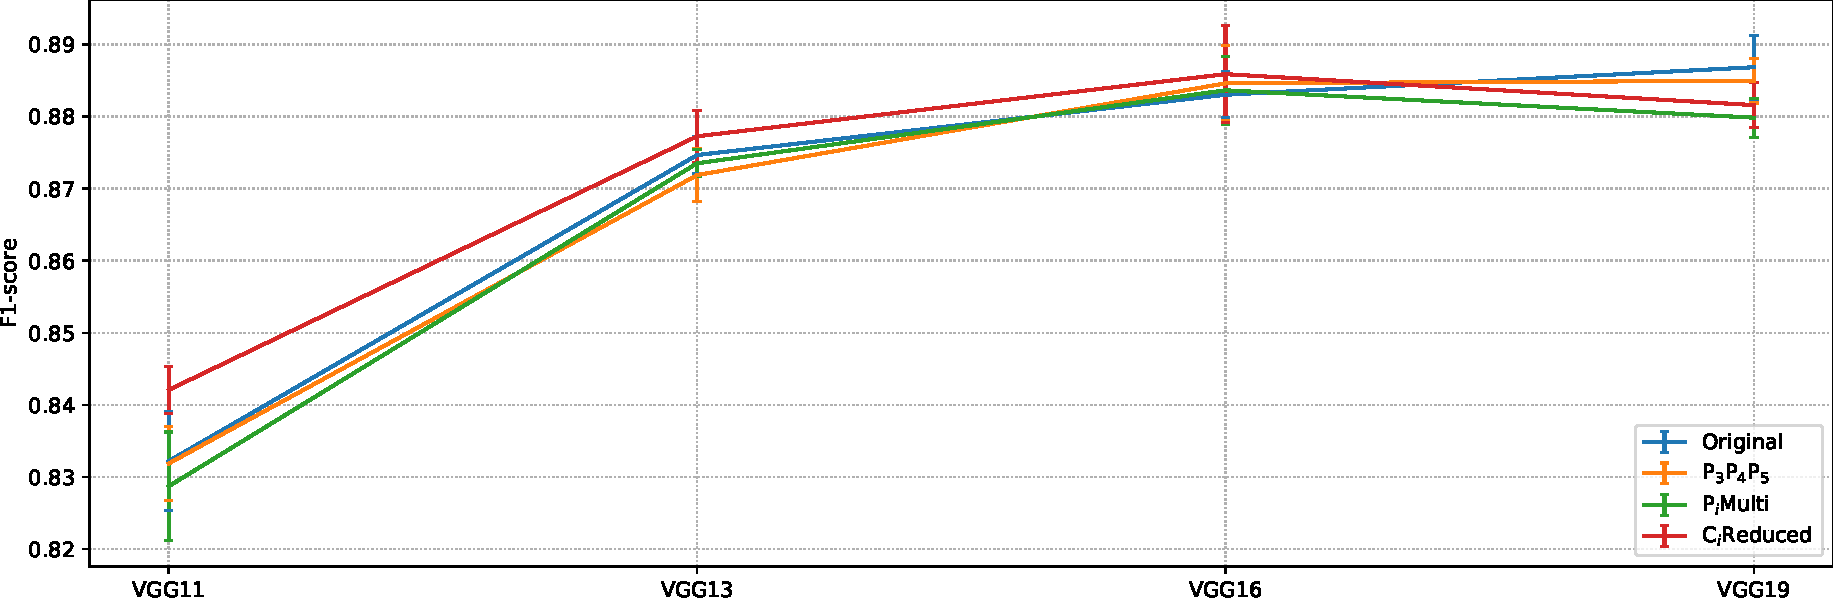
\includegraphics[width=\textwidth]{figures/ch3/fig8.pdf}
  \caption{Comparative results of F1-score versus the four VGG models, for each proposed RetinaNet model. Results were averaged over 10 times.}
  \label{fig8}
\end{figure}

\begin{table}[!htb]
  \centering
  \resizebox{0.75\textwidth}{!}{
  \begin{tabular}{ccccc}
  \toprule
  \textbf{F1-score} & \textbf{VGG11} & \textbf{VGG13} & \textbf{VGG16} & \textbf{VGG19} \\
  \midrule
  Original (202)							&	0.832$\pm$0.007		&	0.875$\pm$0.003		& 	0.883$\pm$0.003	&	\textbf{0.887$\pm$0.004}\\
  $\text{P}_3\text{P}_4\text{P}_5$ (202)		&	0.832$\pm$0.005		&	0.872$\pm$0.004		& 	0.885$\pm$0.005	&	0.885$\pm$0.003\\
  $\text{P}_\text{i}\text{Multi}$ (202)			&	0.829$\pm$0.008		&	0.874$\pm$0.002 		& 	0.884$\pm$0.005	&	0.880$\pm$0.003\\
  \textbf{$\text{C}_\text{i}\text{Reduced}$} (202) &	\textbf{0.842$\pm$0.003}	&	\textbf{0.877$\pm$0.004}	&	\textbf{0.886$\pm$0.007}	&	0.882$\pm$0.003\\
  \bottomrule
  \end{tabular}
  }
  \caption{Indicative values of F1-score for the selected four VGG models, for each proposed RetinaNet model (\fref{fig8}). Parentheses indicate the input resolution.}
  \label{tab4}
\end{table}

Concerning the side-network, apart from $\text{C}_\text{i}\text{Reduced}$, the rest RetinaNet deployments, did not demonstrate any striking difference. Under most VGG architectures, $\text{C}_\text{i}\text{Reduced}$ outperformed notably the rest of the architectures, especially in AP. This observation manifests that the problem under study is not affected considerably by the complexity of the side-network in ways such as: integration of high-level semantic feature maps, attaching separate classifier-regressor heads or increasing the depth. Nonetheless, a lighter version of the original RetinaNet, inspired by the SSD pipeline, addresses the apple detection problem through the ACFR dataset satisfactorily.

\tref{tab5} shows that inference time scales with the depth of the model upon increasing the total parameters, apart from the VGG16 and VGG19, which have the same inference time. Lightweight RetinaNet - $\text{C}_\text{i}\text{Reduced}$, holds the highest detection rates among the rest models, as expected.

%$\text{C}_\text{i}\text{Reduced}$ is the lightest model with the smallest memory footprint among the rest; only 19.8M parameters coupled with VGG16, while VGG19 has 20M parameters itself. It achieves high rate detections while maintaining the highest AP = 0.936.

\begin{table}[!htb]
  \centering
  \resizebox{0.8\textwidth}{!}{
  \begin{tabular}{ccccc}
  \toprule
  \textbf{Inference time (FPS)}	  			& \textbf{VGG11} 	& \textbf{VGG13} 	& \textbf{VGG16} 	& \textbf{VGG19} \\
  \midrule
  Original (202)							&	61.0$\pm$3.5		&	58.8$\pm$3.0		& 	55.3$\pm$2.5	&	55.3$\pm$2.5\\
  $\text{P}_3\text{P}_4\text{P}_5$ (202) 		&	71.1$\pm$3.3		&	69.1$\pm$2.5		& 	67.3$\pm$2.0	&	67.3$\pm$2.0\\
  $\text{P}_\text{i}\text{Multi}$ (202)			&	67.8$\pm$4.4		&	67.3$\pm$3.1		& 	65.2$\pm$2.7	&	65.2$\pm$2.7\\
  \textbf{$\text{C}_\text{i}\text{Reduced}$} (202)	& \textbf{74.0$\pm$5.1}	& \textbf{71.1$\pm$4.5}	& \textbf{65.2$\pm$4.3} 	& \textbf{65.2$\pm$4.3}\\
  \bottomrule
  \end{tabular}
  }
  \caption{Inference time for every VGG. Detection rates depend heavily on the No. of parameters of the model and the input resolution. However, the transition from VGG16 to VGG19 did not show any change.}
  \label{tab5}
\end{table}

All VGG models were initialised upon the pre-trained ImageNet weights. Training with random weight initialisation delayed convergence, but did not show any improvement in the results as demonstrated in \cite{bargoti2017deep}. Transfer learning among the VGG models, that is transferring the weights progressively from VGG11 to VGG19 (\cite{simonyan2014very}), did not show any other improvement in performance rather than saving training from a couple of epochs ($\sim3$ minutes with a resolution of $202\times308$).


\section{Performance - Training Size Relation}
This section presents a performance analysis of RetinaNet - $\text{C}_\text{i}\text{Reduced}$ (202)	over the size of the training dataset. For each training subset, N samples were drawn from the training dataset randomly, without replacement (negative samples were discarded). The subsets were created once and then used for 10 training sessions each. The models were prone to overfitting, particularly those trained on small datasets; thus, early stopping was implemented to obtain the maximum possible performance. \fref{fig9} makes evident, that the model performs satisfactorily already from the first 10 samples. Furthermore, 200 to 500 samples are enough to achieve state-of-the-art performance. From the first 6 samples, RetinaNet outperforms Faster R-CNN in the work of \cite{bargoti2017deep} by 0.1 in every consecutive training subset.

 \begin{figure}[!htb]
  \centering
  \subfigure[]{
    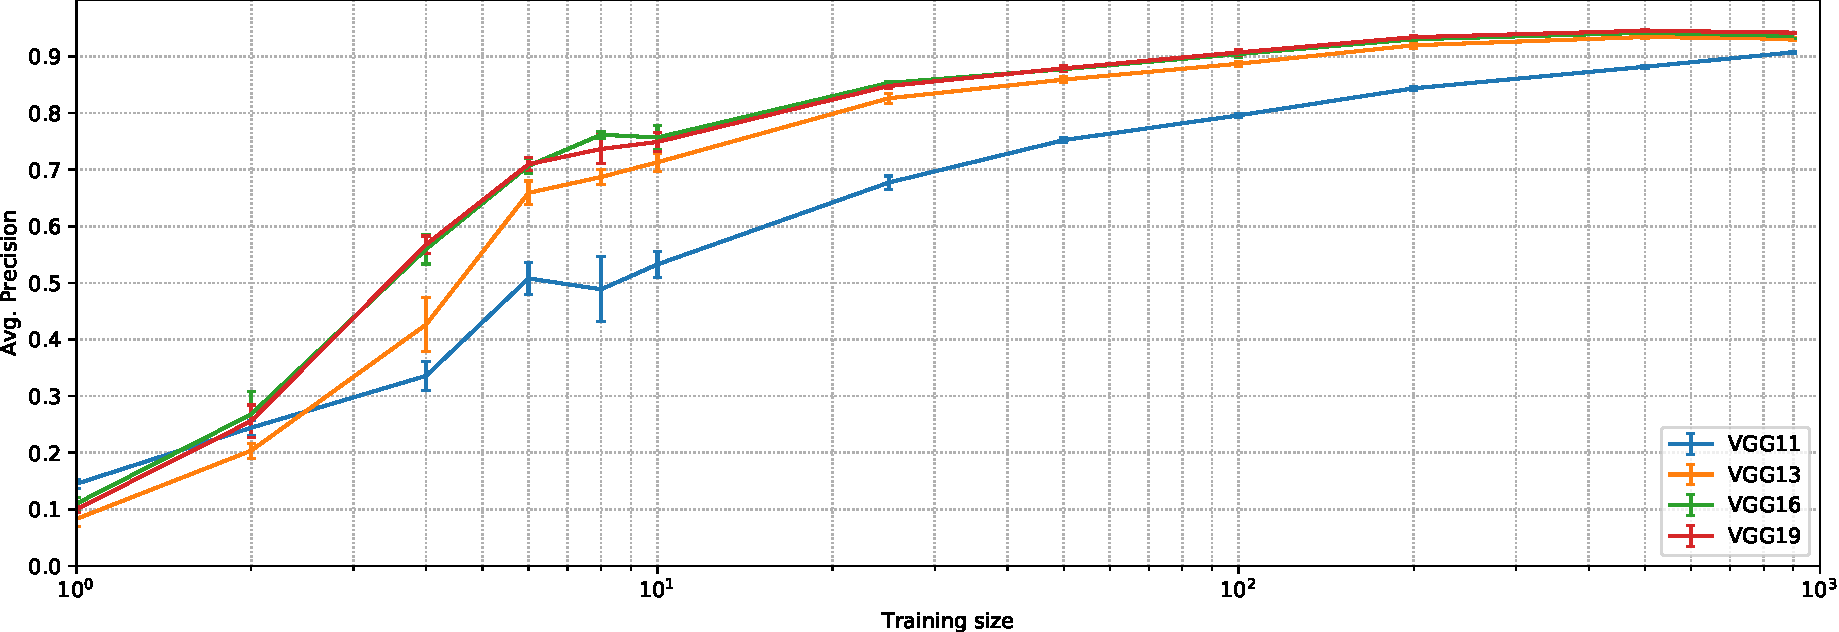
\includegraphics[width=0.9\textwidth]{figures/ch3/fig9_1.pdf}
    \label{fig9_1}
  }
  \subfigure[]{
    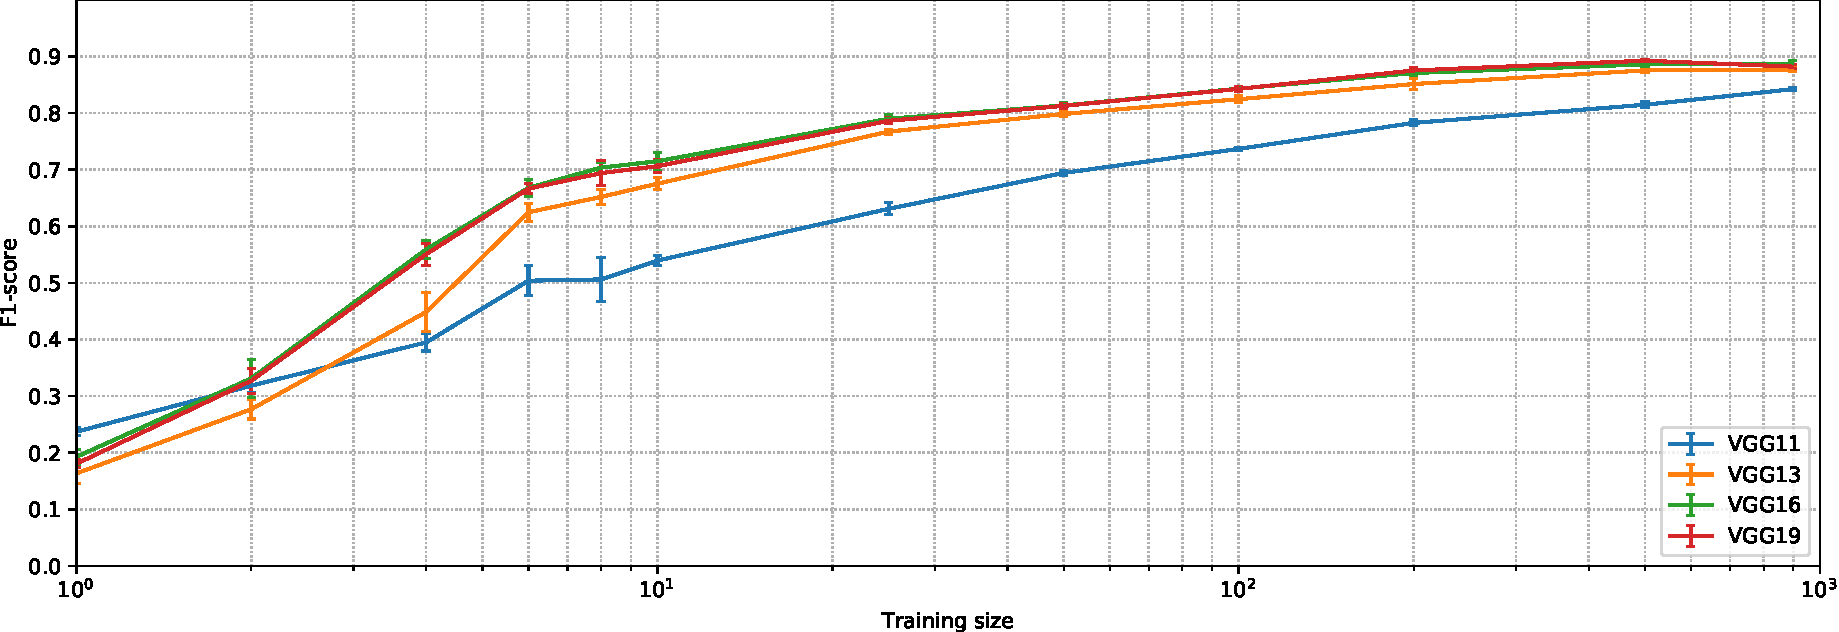
\includegraphics[width=0.9\textwidth]{figures/ch3/fig9_2.pdf}
    \label{fig9_2}
  }
  \caption{Avg. Precision and F1-score as a function of the number of training images on RetinaNet - $\text{C}_\text{i}\text{Reduced}$ (202), for each VGG network.}
  \label{fig9}
\end{figure}

Regarding backbone's network depth, VGG16 and VGG19 show their superiority over the rest architectures consistently. Another interesting feature of \fref{fig9} is that in training sessions consisting more than 10 samples, VGG11 attained the same performance with VGG16-19 only by decupling the dataset.

\section{Peak Detection and Evaluation}
To obtain maximum performance, RetinaNet - $\text{C}_\text{i}\text{Reduced}$ was trained on VGG16, using three resolutions ($202\times308$, $512\times781$ and $800\times1220$) as described in section \ref{training_details}, with F1-score being as the primary evaluation metric. Models presented here were trained initially on the training dataset and then both on the training and validation dataset, while being evaluated on the held-out testing dataset.

\begin{savenotes}
\begin{table}[!htb]
  \centering
  \resizebox{0.8\textwidth}{!}{
  \begin{tabular}{ccccc}
  \toprule
  \textbf{$(\text{IoU}=0.2 , \text{NMS} = 0.3)$}	& \textbf{AP} 	& \textbf{F1} 	& \textbf{mIoU} 	&  \textbf{$\Delta E$} \\
  \midrule
  train. (202)					&	0.948	&	0.895		& 	0.793	&	0.099\\
  train. (512) 					&	0.953	&	0.903		& 	0.814	&	0.040\\
  train. (800)					&	0.952	&	0.903		& 	0.829	&	\textbf{0.016}\\
  train. + val. (202)				&	0.949	&	0.895		& 	0.807	&	0.081\\
  train. + val. (512)				&	0.954	&	0.905		& 	0.824	&	0.038\\
  train. + val. (800)				&	0.953	&	\textbf{0.907}	& 	0.835	&	0.025\\
  \midrule
  Faster R-CNN (ZF) [1]\footnote{[1]: \cite{bargoti2017deep}}		& 	-		&	0.892		&	-		&	-\\
  Faster R-CNN (VGG16) [1]								& 	-		&	0.904		&	-		&	-\\
  Faster R-CNN (VGG16) [2]\footnote{[2]: \cite{liang2018apple}}	& 	-		&	0.879		&	-		&	-\\
  \midrule
  SSD (300) [2]												& 	-		&	0.883		&	-		&	-\\
  SSD (500) [2]												& 	-		&	0.890		&	-		&	-\\
  \bottomrule
  \end{tabular}
  }
  \caption{Comparing performance of RetinaNet - $\text{C}_\text{i}\text{Reduced}$ (VGG16), trained on the training and on the combined training - validation set, with the state-of-the-art models. Parentheses indicate resolutions.}
  \label{tab6}
\end{table}
\end{savenotes}

\tref{tab6} shows that performance increases with resolution, with the best model achieving a maximum F1-score of \textbf{0.907}, outperforming the previous state-of-the-art model (\cite{bargoti2017deep}). \cite{liang2018apple} gave more emphasis on real-time detection achieving 43.47 FPS using the SSD(300).

RetinaNet - $\text{C}_\text{i}\text{Reduced}$(VGG16), beaten SSD in performance and inference time by using even smaller resolution. A resolution of 800 improved performance, in terms of F1-score by $\sim1\%$, but with a considerable drop in training time versus the smaller resolution of 202. Specifically, models trained on the original image dimensions ($202\times308$), required x4 times less time to train in comparison to the ones that used ($800\times1220$) and also, they had x5.5 times less inference time (12.6FPS vs 65.2 FPS).

Moreover, from \tref{tab6} it can be seen that, while the IoU threshold was set equal to 0.2, as in the previous sections, the mean IoU between ground truths and predictions is quite high, making very accurate localisations.

\begin{figure}[!htb]
  \centering
  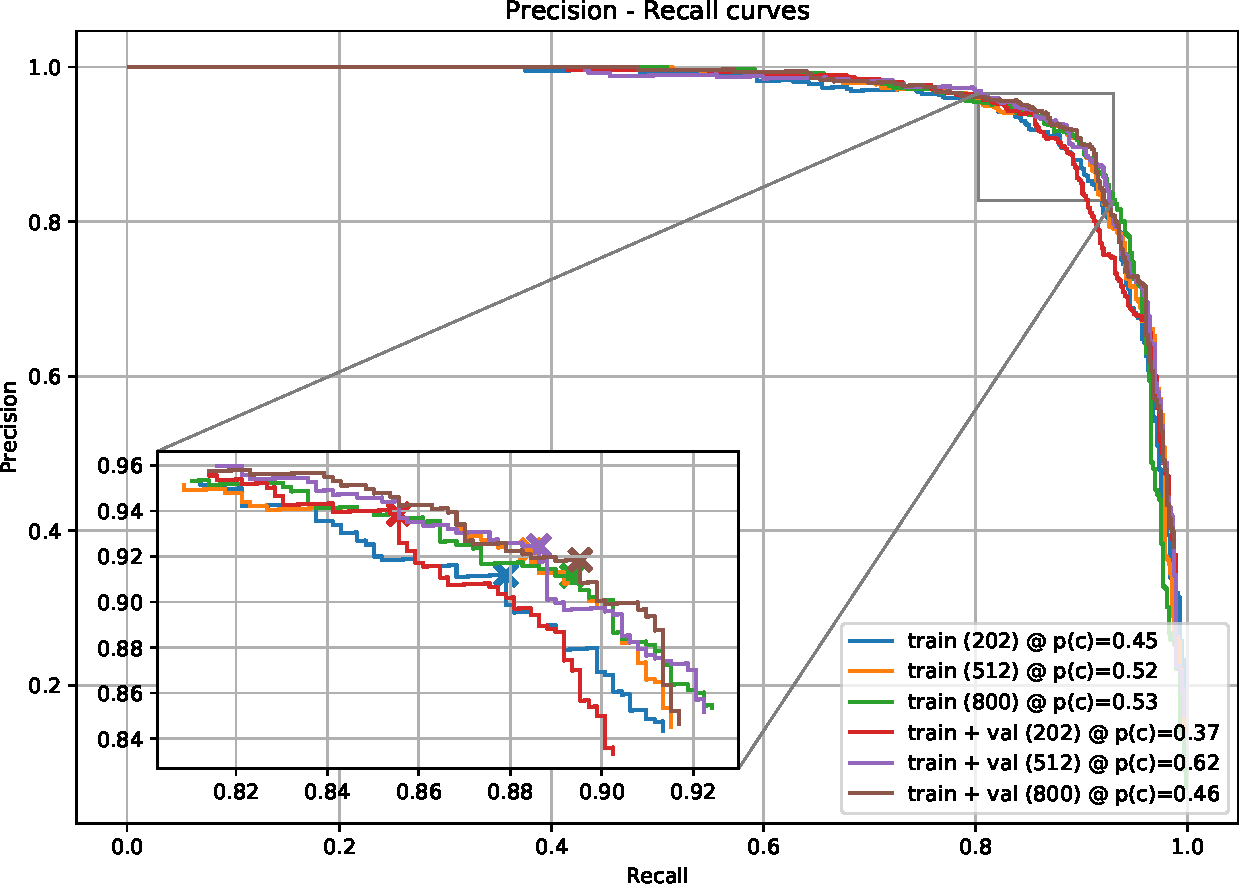
\includegraphics[width=\textwidth]{figures/ch3/fig10.pdf}
  \caption{Precision - Recall curves for the RetinaNet - $\text{C}_\text{i}\text{Reduced}$ (VGG16). AP is defined by the area under the curve, while F1-score is the point on the curve where Precision and Recall take maximum values.}
  \label{fig10}
\end{figure} 

\fref{fig10} illustrates the precision-recall curves of the trained models presented in \tref{tab6}. All models maintain very high precision for all recall levels. Precision stays around 1.0 for most recall values and starts to drop after recall takes higher values than 0.8.

\subsection{Performance at Various IoU Thresholds}
\subsection{Performance at Various NMS Thresholds}
\subsection{Counting}
The dataset does not specify any structure among the trellised trees in the pictures, thus structured yield estimation in the orchard block is impossible. However, $\Delta E$ represents overall count estimates, by using the normalised absolute error over the total number of instances in the dataset. $\Delta E$ seems to take smaller values as F1-score increase, giving an unstructured yield estimate for the whole dataset through the total number of predictions. Instead of tuning the detection confidence threshold to minimise $\Delta E$, it was optimised to take the maximum value, while keeping F1-score unchanged.
